\section{Convolutional Neural Networks}
\label{convolutional_neural_networks}

Neuronale Netze \bzw{} Deep-Learning gehören zu den derzeit besten und beliebtesten Lösungen zu Problemen der Bild- oder Spracherkennung~\cite{Nielsen}.
Dabei lernt \bzw{} approximiert das Netz durch eine Anpassung ihrer Parameter über einer Menge an Trainingsbeispielen eine Funktion, sodass die Trainingsbeispiele auf ihre gewünschte Ausgabe abbilden und auch für unbekannte Eingaben zuverlässige Vorhersagen getroffen werden können.
Neuronale Netze sind daher größtenteils in dem Bereich des \emph{überwachten maschinellen Lernens} anzuordnen.
Ein Netz, welches lediglich die Trainingsmenge lernt, aber über der Trainingsmenge hinausgehende Daten nicht beschreiben kann, wird als ein \emph{überangepasstes} (\engl{} \emph{overfitted}) Netz bezeichnet~\cite{Nielsen}.

Ein \emph{neuronales Netz} besteht aus einer beliebigen Anzahl miteinander verbundener \emph{Neuronen}.
Neuronen sind üblicherweise mit anderen Neuronen in sequentiellen \emph{Schichten} \bzw{} \emph{Ebenen} angeordnet.
Die erste Schicht eines neuronalen Netzes wird als \emph{Eingabe}- und die letzte Schicht als  \emph{Ausgabeschicht} bezeichnet.
Schichten zwischen Ein- und Ausgabe heißen \emph{versteckt} (\engl{} \emph{hidden}).
Als \emph{Deep-Learning} wird ein Netz mit mindestens zwei versteckten Schichten verstanden.
Die einfachste Form eines neuronalen Netzes ist das \emph{Feedforward}-Netz, bei der jedes Neuron einer Schicht mit allen Neuronen der darauffolgenden Schicht verbunden ist.
Die Schichten eines Feedforward-Netzes werden deshalb auch als \emph{vollverbunden} (\engl{} \emph{fully-connected}) betitelt.
Abbildung~\ref{fig:feedforward} zeigt ein Beispiel eines solchen Netzes mit drei Schichten.
\begin{figure}[t]
\centering
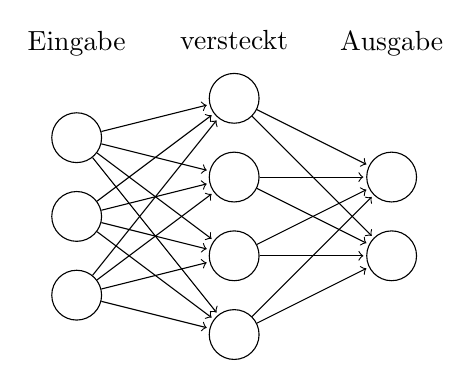
\begin{tikzpicture}
  \tikzstyle{node}=[circle,draw, minimum width=18pt, inner sep=0pt, fill=white]
  \tikzstyle{edge}=[->, shorten >= 1pt]

  \node[rectangle, inner sep=0pt] at (-2, 2.2) {Eingabe};
  \node[rectangle, inner sep=1pt] at (0,  2.24) {versteckt};
  \node[rectangle, inner sep=0pt] at (2,  2.2) {Ausgabe};

  \node[node] (a1) at (-2, -1) {};
  \node[node] (a2) at (-2, 0)  {};
  \node[node] (a3) at (-2, 1)  {};

  \node[node] (b1) at (0, -1.5) {};
  \node[node] (b2) at (0, -0.5) {};
  \node[node] (b3) at (0, 0.5)  {};
  \node[node] (b4) at (0, 1.5)  {};

  \node[node] (c1) at (2, -0.5) {};
  \node[node] (c2) at (2, 0.5)  {};

  \path[edge] (a1) edge (b1);
  \path[edge] (a1) edge (b2);
  \path[edge] (a1) edge (b3);
  \path[edge] (a1) edge (b4);
  \path[edge] (a2) edge (b1);
  \path[edge] (a2) edge (b2);
  \path[edge] (a2) edge (b3);
  \path[edge] (a2) edge (b4);
  \path[edge] (a3) edge (b1);
  \path[edge] (a3) edge (b2);
  \path[edge] (a3) edge (b3);
  \path[edge] (a3) edge (b4);
  \path[edge] (b1) edge (c1);
  \path[edge] (b1) edge (c2);
  \path[edge] (b2) edge (c1);
  \path[edge] (b2) edge (c2);
  \path[edge] (b3) edge (c1);
  \path[edge] (b3) edge (c2);
  \path[edge] (b4) edge (c1);
  \path[edge] (b4) edge (c2);
\end{tikzpicture}
\caption[Feedforward-Netz]{Beispiel eines Feedforward-Netzes mit drei vollverbundenen Schichten von einer Eingabe mit drei Neuronen zu einer Ausgabe mit zwei Neuronen und einer dazwischenliegenden versteckten Schicht.}
\label{fig:feedforward}
\end{figure}

Andere Netzvarianten erlauben \zB{} Schleifen, Rückwärtskanten oder das Überspringen einer Schicht~\cite{Nielsen}.

Ein Neuron besitzt genau einen reellen Wert, der sich aus den Neuronen der vorherigen Schicht erschließt.
Die $t$-te Neuronenschicht lässt sich folglich als ein Vektor $\ve{x}^{\left(t\right)} \in \gls{R}^{N^{\left(t\right)}}$ auffassen, wobei $N^{\left(t\right)} \in \gls{N}$ die Anzahl der Neuronen in der $t$-ten Schicht beschreibt.
Zu jeder Kante existiert zusätzlich ein Gewicht, welches den Anteil des Neurons zu dessen verbundenen Neuron angibt.
Damit lassen sich die Neuronenwerte der $\left(t+1\right)$-ten Schicht über
\begin{equation*}
  \ve{x}^{\left(t+1\right)} \coloneqq \gls{W}^{\left(t+1\right)}\ve{x}^{\left(t\right)}
\end{equation*}
definieren, wobei $\gls{W}^{\left(t+1\right)} \in \gls{R}^{N^{\left(t+1\right)} \times N^{\left(t\right)}}$ eine \emph{Gewichtsmatrix} der Kanten beschreibt, sodass $\gls{W}^{\left(t+1\right)}_{ji} \in \gls{R}$ das Gewicht der Kante des $i$-ten Neurons in der $t$-ten Schicht zu dem $j$-ten Neuron der $\left(t+1\right)$-ten Schicht angibt.
Zusätzlich zu den Gewichten existert zu jedem Neuron in der $t$-ten Schicht außer der Eingabeschicht ein \emph{Bias} $\gls{b}^{\left(t\right)} \in \gls{R}^{N^{\left(t\right)}}$.
Mit einer elementweisen Anwendung einer nicht-linearen \emph{Aktivierungsfunktion} $\gls{act} \colon \gls{R} \to \gls{R}$ ergibt sich damit die finale Version der Neuronenwerte der $\left(t+1\right)$-ten Schicht als
\begin{equation*}
  \ve{x}^{\left(t+1\right)} \coloneqq \gls{act} \left(\gls{W}^{\left(t+1\right)}\ve{x}^{\left(t\right)} + \gls{b}^{\left(t+1\right)} \right).
\end{equation*}
Als Aktivierungsfunktion kommt dabei \bspw{} die nicht-lineare \emph{Sigmoidfunktion} $\mathrm{sig}\left(z\right) \coloneqq 1 / \left(1 + \exp\left(-z\right)\right)$ oder die \emph{Rectified Linear Unit (ReLU)}-Funktion $\gls{relu}\left(z\right) \coloneqq \max \left(z, 0\right)$ zum Einsatz~\cite{Nielsen}.
Die Menge der Gewichte $\mathcal{W} \coloneqq {\left\{\gls{W}^{\left(t\right)}\right\}}_{t=2}^T$ sowie die Menge der Biaswerte $\mathcal{B} \coloneqq {\left\{\gls{b}^{\left(t\right)}\right\}}_{t=2}^T$ der $T \in \gls{N}$ vielen Schichten werden die \emph{Parameter} des Netzes genannt, über dessen Anpassung das Netz trainiert wird.
Diese Werte werden dabei sequentiell über einer kleinen Eingabemenge $\mathcal{X}$ mit den Eingaben $\ve{x} \in \mathcal{X}$ so angepasst, dass eine \emph{Kostenfunktion} minimiert wird.
Die Größe der Menge $\mathcal{X}$ wird dabei als \emph{Batch-Size} betitelt~\cite{Nielsen}.
Ein Beispiel einer Kostenfunktion ist die \emph{quadratische Kostenfunktion}, die über
\begin{equation}
  C\left(\mathcal{X}, \mathcal{W}, \mathcal{B}\right) \coloneqq \frac{1}{2\left|\mathcal{X}\right|} \sum_{\ve{x} \in \mathcal{X}} {\left\| \ve{y} - \ve{y}^{\prime} \right\|}_2^2
  \label{eq:quadratische_kostenfunktion}
\end{equation}
definiert ist, wobei \ve{y} die Ausgabe des Netzes und $\ve{y}^{\prime}$ die erwartete Ausgabe \bzgl{} \ve{x} beschreibt~\cite{Nielsen}.
Die implizit durch das Netz gegebenen Werte $\mathcal{W}$ und $\mathcal{B}$ werden dabei oft weggelassen, sodass wir lediglich $C\left(\mathcal{X}\right)$ schreiben.
$C$ zeichnet sich dabei als Kostenfunktion aus, denn sie ist für alle Eingaben stets positiv und wird umso kleiner, je ähnlicher \ve{y} und $\ve{y}^{\prime}$ werden.
Die Anpassung der Parameter des Netzes erfolgt über die sukzessive Eingabe einer Menge $\mathcal{X}$ in das Netz und der Berechnung eines negativen Gradienten in Richtung des steilsten Abstieges von $C$.
Formal betrachtet entspricht der Gradient der Kostenfunktion $C$ dem Vektor der partiellen Ableitungen
\begin{equation*}
  \nabla C \coloneqq {\left[\frac{\partial C}{\partial w_i}, \ldots, \frac{\partial C}{\partial b_j}, \ldots \right]}^{\top}
\end{equation*}
aller Gewichte $w_i$ und aller Biaswerte $b_j$ des Netzes~\cite{Nielsen}.
Durch die Anpassung der Gewichte und Biaswerte des Netzes über
\begin{equation*}
  w_i \rightarrow w^{\prime}_i = w_i - \gls{learning}\frac{\partial C}{\partial w_i}
  \qquad
  \text{und}
  \qquad
  b_j \rightarrow b^{\prime}_j = b_j - \gls{learning}\frac{\partial C}{\partial b_j}
\end{equation*}
wird die Kostenfunktion $C$ minimiert, wobei $\gls{learning} \in \gls{R+}$ der \emph{Lernrate}, \dhe{} der gewählten Schrittweite, entlang des negativen Gradienten entspricht~\cite{Nielsen}.
Üblicherweise wird dabei \gls{learning} so gewählt, dass das Netz nicht zu langsam trainiert, aber dennoch eine gute Approximation erreicht wird und erfordert in der Regel eine manuelle Anpassung.
Die Berechnung des Gradienten $\nabla C$ wird dabei aus Berechnungsgründen nicht für alle, sondern lediglich für Eingaben einer zufällig ausgewählten Untermenge von $\mathcal{X}$ durchgeführt und daraus dessen Durchschnitt gebildet, welcher stochastisch gesehen in etwa dem realen Gradienten über allen Eingaben entspricht (\emph{stochastischer Gradientenabstieg})~\cite{Nielsen}.
Zur Berechnung des Gradienten der Kostenfunktion $C$ kommt dabei der effiziente \emph{Backpropagation}-Algorithmus zum Einsatz, der es ermöglicht die optimierten Werte der Parameter nach einem Trainingsschritt zu ermitteln, indem der Fehler zwischen der Ausgabe des Netzes und der erwarteten Ausgabe über die Ausgabe- zur Eingabeschicht zurück propagiert wird~\cite{backpropagation}.
Aus den Fehlern der einzelnen Neuronen kann damit schließlich der Gradient $\nabla C$ berechnet werden (\vgl{}~\cite{Nielsen}).

Der Prozess des Trainings eines neuronalen Netzes, \dhe{} die Anpassung seiner Parameter zur Minimierung der Kostenfunktion, wird dabei solange wiederholt, bis $\nabla C$ ein lokales Minimum erreicht.
Ein einmaliges Durchlaufen aller Eingaben der Eingabemenge wird dabei als \emph{Epoche} bezeichnet~\cite{Nielsen}.
\\\\
Eine Spezialform eines neuronalen Netz ist das \emph{\gls{CNN}}, welches hauptsächlich in der Bild- und Spracherkennung zum Einsatz kommt und seinen Namen aufgrund der \emph{Faltung} seiner Eingabe mit einem \emph{Filter} erhält.~\cite{cnn}.
Entgegen eines Feedforward-Netzes, welches stets einen Vektor als Eingabe erwartet, arbeitet ein \gls{CNN} auf den originalen Bilddaten, \dhe{} einer Menge zweidimensionaler Matrizen, und ermöglicht so, dass dessen räumliche Struktur beim Lernen berücksichtigt wird~\cite{Nielsen}.
Dabei wird ein Neuron nicht mehr mit allen Neuronen der vorherigen Schicht, sondern nur noch mit einer Teilmenge dieser innerhalb eines Fensters um das Neuron verbunden.
Dieses Fenster wird auch oft, angelehnt an die Rezeptoren eines Auges, \emph{rezeptives Feld} (\engl{} \emph{Receptive-Field}) genannt~\cite{cnn}.
Die Größe des Receptive-Fields, \zB{} $5 \times 5$, wird dabei als \emph{Filtergröße} bezeichnet.
Abbildung~\ref{fig:cnn} veranschaulicht die Vernetzung der Neuronen durch ein Receptive-Field.
\section{Convolutional Neural Networks}
\label{convolutional_neural_networks}

Neuronale Netze \bzw{} Deep-Learning gehören zu den derzeit besten und beliebtesten Lösungen zu Problemen der Bild- oder Spracherkennung~\cite{Nielsen}.
Dabei lernt \bzw{} approximiert das Netz durch eine Anpassung ihrer Parameter über einer Menge an Trainingsbeispielen eine Funktion, sodass die Trainingsbeispiele auf ihre gewünschte Ausgabe abbilden und auch für unbekannte Eingaben zuverlässige Vorhersagen getroffen werden können.
Neuronale Netze sind daher größtenteils in dem Bereich des \emph{überwachten maschinellen Lernens} anzuordnen.
Ein Netz, welches lediglich die Trainingsmenge lernt, aber über der Trainingsmenge hinausgehende Daten nicht beschreiben kann, wird als ein \emph{überangepasstes} (\engl{} \emph{overfitted}) Netz bezeichnet~\cite{Nielsen}.

Ein \emph{neuronales Netz} besteht aus einer beliebigen Anzahl miteinander verbundener \emph{Neuronen}.
Neuronen sind üblicherweise mit anderen Neuronen in sequentiellen \emph{Schichten} \bzw{} \emph{Ebenen} angeordnet.
Die erste Schicht eines neuronalen Netzes wird als \emph{Eingabe}- und die letzte Schicht als  \emph{Ausgabeschicht} bezeichnet.
Schichten zwischen Ein- und Ausgabe heißen \emph{versteckt} (\engl{} \emph{hidden}).
Als \emph{Deep-Learning} wird ein Netz mit mindestens zwei versteckten Schichten verstanden.
Die einfachste Form eines neuronalen Netzes ist das \emph{Feedforward}-Netz, bei der jedes Neuron einer Schicht mit allen Neuronen der darauffolgenden Schicht verbunden ist.
Die Schichten eines Feedforward-Netzes werden deshalb auch als \emph{vollverbunden} (\engl{} \emph{fully-connected}) betitelt.
Abbildung~\ref{fig:feedforward} zeigt ein Beispiel eines solchen Netzes mit drei Schichten.
\begin{figure}[t]
\centering
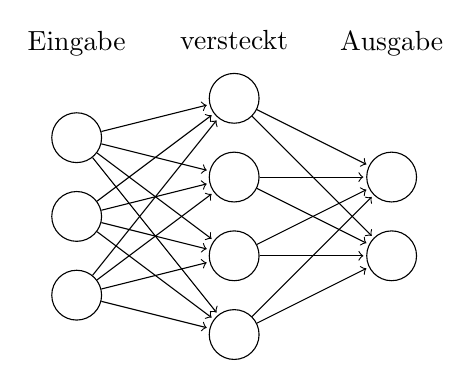
\begin{tikzpicture}
  \tikzstyle{node}=[circle,draw, minimum width=18pt, inner sep=0pt, fill=white]
  \tikzstyle{edge}=[->, shorten >= 1pt]

  \node[rectangle, inner sep=0pt] at (-2, 2.2) {Eingabe};
  \node[rectangle, inner sep=1pt] at (0,  2.24) {versteckt};
  \node[rectangle, inner sep=0pt] at (2,  2.2) {Ausgabe};

  \node[node] (a1) at (-2, -1) {};
  \node[node] (a2) at (-2, 0)  {};
  \node[node] (a3) at (-2, 1)  {};

  \node[node] (b1) at (0, -1.5) {};
  \node[node] (b2) at (0, -0.5) {};
  \node[node] (b3) at (0, 0.5)  {};
  \node[node] (b4) at (0, 1.5)  {};

  \node[node] (c1) at (2, -0.5) {};
  \node[node] (c2) at (2, 0.5)  {};

  \path[edge] (a1) edge (b1);
  \path[edge] (a1) edge (b2);
  \path[edge] (a1) edge (b3);
  \path[edge] (a1) edge (b4);
  \path[edge] (a2) edge (b1);
  \path[edge] (a2) edge (b2);
  \path[edge] (a2) edge (b3);
  \path[edge] (a2) edge (b4);
  \path[edge] (a3) edge (b1);
  \path[edge] (a3) edge (b2);
  \path[edge] (a3) edge (b3);
  \path[edge] (a3) edge (b4);
  \path[edge] (b1) edge (c1);
  \path[edge] (b1) edge (c2);
  \path[edge] (b2) edge (c1);
  \path[edge] (b2) edge (c2);
  \path[edge] (b3) edge (c1);
  \path[edge] (b3) edge (c2);
  \path[edge] (b4) edge (c1);
  \path[edge] (b4) edge (c2);
\end{tikzpicture}
\caption[Feedforward-Netz]{Beispiel eines Feedforward-Netzes mit drei vollverbundenen Schichten von einer Eingabe mit drei Neuronen zu einer Ausgabe mit zwei Neuronen und einer dazwischenliegenden versteckten Schicht.}
\label{fig:feedforward}
\end{figure}

Andere Netzvarianten erlauben \zB{} Schleifen, Rückwärtskanten oder das Überspringen einer Schicht~\cite{Nielsen}.

Ein Neuron besitzt genau einen reellen Wert, der sich aus den Neuronen der vorherigen Schicht erschließt.
Die $t$-te Neuronenschicht lässt sich folglich als ein Vektor $\ve{x}^{\left(t\right)} \in \gls{R}^{N^{\left(t\right)}}$ auffassen, wobei $N^{\left(t\right)} \in \gls{N}$ die Anzahl der Neuronen in der $t$-ten Schicht beschreibt.
Zu jeder Kante existiert zusätzlich ein Gewicht, welches den Anteil des Neurons zu dessen verbundenen Neuron angibt.
Damit lassen sich die Neuronenwerte der $\left(t+1\right)$-ten Schicht über
\begin{equation*}
  \ve{x}^{\left(t+1\right)} \coloneqq \gls{W}^{\left(t+1\right)}\ve{x}^{\left(t\right)}
\end{equation*}
definieren, wobei $\gls{W}^{\left(t+1\right)} \in \gls{R}^{N^{\left(t+1\right)} \times N^{\left(t\right)}}$ eine \emph{Gewichtsmatrix} der Kanten beschreibt, sodass $\gls{W}^{\left(t+1\right)}_{ji} \in \gls{R}$ das Gewicht der Kante des $i$-ten Neurons in der $t$-ten Schicht zu dem $j$-ten Neuron der $\left(t+1\right)$-ten Schicht angibt.
Zusätzlich zu den Gewichten existert zu jedem Neuron in der $t$-ten Schicht außer der Eingabeschicht ein \emph{Bias} $\gls{b}^{\left(t\right)} \in \gls{R}^{N^{\left(t\right)}}$.
Mit einer elementweisen Anwendung einer nicht-linearen \emph{Aktivierungsfunktion} $\gls{act} \colon \gls{R} \to \gls{R}$ ergibt sich damit die finale Version der Neuronenwerte der $\left(t+1\right)$-ten Schicht als
\begin{equation*}
  \ve{x}^{\left(t+1\right)} \coloneqq \gls{act} \left(\gls{W}^{\left(t+1\right)}\ve{x}^{\left(t\right)} + \gls{b}^{\left(t+1\right)} \right).
\end{equation*}
Als Aktivierungsfunktion kommt dabei \bspw{} die nicht-lineare \emph{Sigmoidfunktion} $\mathrm{sig}\left(z\right) \coloneqq 1 / \left(1 + \exp\left(-z\right)\right)$ oder die \emph{Rectified Linear Unit (ReLU)}-Funktion $\gls{relu}\left(z\right) \coloneqq \max \left(z, 0\right)$ zum Einsatz~\cite{Nielsen}.
Die Menge der Gewichte $\mathcal{W} \coloneqq {\left\{\gls{W}^{\left(t\right)}\right\}}_{t=2}^T$ sowie die Menge der Biaswerte $\mathcal{B} \coloneqq {\left\{\gls{b}^{\left(t\right)}\right\}}_{t=2}^T$ der $T \in \gls{N}$ vielen Schichten werden die \emph{Parameter} des Netzes genannt, über dessen Anpassung das Netz trainiert wird.
Diese Werte werden dabei sequentiell über einer kleinen Eingabemenge $\mathcal{X}$ mit den Eingaben $\ve{x} \in \mathcal{X}$ so angepasst, dass eine \emph{Kostenfunktion} minimiert wird.
Die Größe der Menge $\mathcal{X}$ wird dabei als \emph{Batch-Size} betitelt~\cite{Nielsen}.
Ein Beispiel einer Kostenfunktion ist die \emph{quadratische Kostenfunktion}, die über
\begin{equation}
  C\left(\mathcal{X}, \mathcal{W}, \mathcal{B}\right) \coloneqq \frac{1}{2\left|\mathcal{X}\right|} \sum_{\ve{x} \in \mathcal{X}} {\left\| \ve{y} - \ve{y}^{\prime} \right\|}_2^2
  \label{eq:quadratische_kostenfunktion}
\end{equation}
definiert ist, wobei \ve{y} die Ausgabe des Netzes und $\ve{y}^{\prime}$ die erwartete Ausgabe \bzgl{} \ve{x} beschreibt~\cite{Nielsen}.
Die implizit durch das Netz gegebenen Werte $\mathcal{W}$ und $\mathcal{B}$ werden dabei oft weggelassen, sodass wir lediglich $C\left(\mathcal{X}\right)$ schreiben.
$C$ zeichnet sich dabei als Kostenfunktion aus, denn sie ist für alle Eingaben stets positiv und wird umso kleiner, je ähnlicher \ve{y} und $\ve{y}^{\prime}$ werden.
Die Anpassung der Parameter des Netzes erfolgt über die sukzessive Eingabe einer Menge $\mathcal{X}$ in das Netz und der Berechnung eines negativen Gradienten in Richtung des steilsten Abstieges von $C$.
Formal betrachtet entspricht der Gradient der Kostenfunktion $C$ dem Vektor der partiellen Ableitungen
\begin{equation*}
  \nabla C \coloneqq {\left[\frac{\partial C}{\partial w_i}, \ldots, \frac{\partial C}{\partial b_j}, \ldots \right]}^{\top}
\end{equation*}
aller Gewichte $w_i$ und aller Biaswerte $b_j$ des Netzes~\cite{Nielsen}.
Durch die Anpassung der Gewichte und Biaswerte des Netzes über
\begin{equation*}
  w_i \rightarrow w^{\prime}_i = w_i - \gls{learning}\frac{\partial C}{\partial w_i}
  \qquad
  \text{und}
  \qquad
  b_j \rightarrow b^{\prime}_j = b_j - \gls{learning}\frac{\partial C}{\partial b_j}
\end{equation*}
wird die Kostenfunktion $C$ minimiert, wobei $\gls{learning} \in \gls{R+}$ der \emph{Lernrate}, \dhe{} der gewählten Schrittweite, entlang des negativen Gradienten entspricht~\cite{Nielsen}.
Üblicherweise wird dabei \gls{learning} so gewählt, dass das Netz nicht zu langsam trainiert, aber dennoch eine gute Approximation erreicht wird und erfordert in der Regel eine manuelle Anpassung.
Die Berechnung des Gradienten $\nabla C$ wird dabei aus Berechnungsgründen nicht für alle, sondern lediglich für Eingaben einer zufällig ausgewählten Untermenge von $\mathcal{X}$ durchgeführt und daraus dessen Durchschnitt gebildet, welcher stochastisch gesehen in etwa dem realen Gradienten über allen Eingaben entspricht (\emph{stochastischer Gradientenabstieg})~\cite{Nielsen}.
Zur Berechnung des Gradienten der Kostenfunktion $C$ kommt dabei der effiziente \emph{Backpropagation}-Algorithmus zum Einsatz, der es ermöglicht die optimierten Werte der Parameter nach einem Trainingsschritt zu ermitteln, indem der Fehler zwischen der Ausgabe des Netzes und der erwarteten Ausgabe über die Ausgabe- zur Eingabeschicht zurück propagiert wird~\cite{backpropagation}.
Aus den Fehlern der einzelnen Neuronen kann damit schließlich der Gradient $\nabla C$ berechnet werden (\vgl{}~\cite{Nielsen}).

Der Prozess des Trainings eines neuronalen Netzes, \dhe{} die Anpassung seiner Parameter zur Minimierung der Kostenfunktion, wird dabei solange wiederholt, bis $\nabla C$ ein lokales Minimum erreicht.
Ein einmaliges Durchlaufen aller Eingaben der Eingabemenge wird dabei als \emph{Epoche} bezeichnet~\cite{Nielsen}.
\\\\
Eine Spezialform eines neuronalen Netz ist das \emph{\gls{CNN}}, welches hauptsächlich in der Bild- und Spracherkennung zum Einsatz kommt und seinen Namen aufgrund der \emph{Faltung} seiner Eingabe mit einem \emph{Filter} erhält.~\cite{cnn}.
Entgegen eines Feedforward-Netzes, welches stets einen Vektor als Eingabe erwartet, arbeitet ein \gls{CNN} auf den originalen Bilddaten, \dhe{} einer Menge zweidimensionaler Matrizen, und ermöglicht so, dass dessen räumliche Struktur beim Lernen berücksichtigt wird~\cite{Nielsen}.
Dabei wird ein Neuron nicht mehr mit allen Neuronen der vorherigen Schicht, sondern nur noch mit einer Teilmenge dieser innerhalb eines Fensters um das Neuron verbunden.
Dieses Fenster wird auch oft, angelehnt an die Rezeptoren eines Auges, \emph{rezeptives Feld} (\engl{} \emph{Receptive-Field}) genannt~\cite{cnn}.
Die Größe des Receptive-Fields, \zB{} $5 \times 5$, wird dabei als \emph{Filtergröße} bezeichnet.
Abbildung~\ref{fig:cnn} veranschaulicht die Vernetzung der Neuronen durch ein Receptive-Field.
\section{Convolutional Neural Networks}
\label{convolutional_neural_networks}

Neuronale Netze \bzw{} Deep-Learning gehören zu den derzeit besten und beliebtesten Lösungen zu Problemen der Bild- oder Spracherkennung~\cite{Nielsen}.
Dabei lernt \bzw{} approximiert das Netz durch eine Anpassung ihrer Parameter über einer Menge an Trainingsbeispielen eine Funktion, sodass die Trainingsbeispiele auf ihre gewünschte Ausgabe abbilden und auch für unbekannte Eingaben zuverlässige Vorhersagen getroffen werden können.
Neuronale Netze sind daher größtenteils in dem Bereich des \emph{überwachten maschinellen Lernens} anzuordnen.
Ein Netz, welches lediglich die Trainingsmenge lernt, aber über der Trainingsmenge hinausgehende Daten nicht beschreiben kann, wird als ein \emph{überangepasstes} (\engl{} \emph{overfitted}) Netz bezeichnet~\cite{Nielsen}.

Ein \emph{neuronales Netz} besteht aus einer beliebigen Anzahl miteinander verbundener \emph{Neuronen}.
Neuronen sind üblicherweise mit anderen Neuronen in sequentiellen \emph{Schichten} \bzw{} \emph{Ebenen} angeordnet.
Die erste Schicht eines neuronalen Netzes wird als \emph{Eingabe}- und die letzte Schicht als  \emph{Ausgabeschicht} bezeichnet.
Schichten zwischen Ein- und Ausgabe heißen \emph{versteckt} (\engl{} \emph{hidden}).
Als \emph{Deep-Learning} wird ein Netz mit mindestens zwei versteckten Schichten verstanden.
Die einfachste Form eines neuronalen Netzes ist das \emph{Feedforward}-Netz, bei der jedes Neuron einer Schicht mit allen Neuronen der darauffolgenden Schicht verbunden ist.
Die Schichten eines Feedforward-Netzes werden deshalb auch als \emph{vollverbunden} (\engl{} \emph{fully-connected}) betitelt.
Abbildung~\ref{fig:feedforward} zeigt ein Beispiel eines solchen Netzes mit drei Schichten.
\begin{figure}[t]
\centering
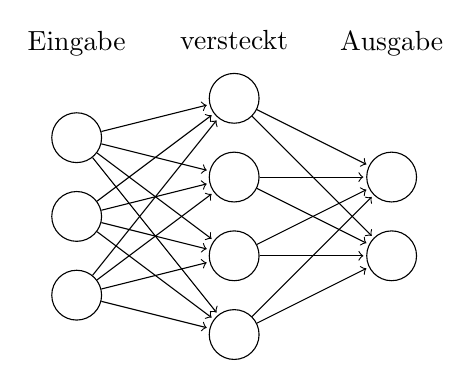
\begin{tikzpicture}
  \tikzstyle{node}=[circle,draw, minimum width=18pt, inner sep=0pt, fill=white]
  \tikzstyle{edge}=[->, shorten >= 1pt]

  \node[rectangle, inner sep=0pt] at (-2, 2.2) {Eingabe};
  \node[rectangle, inner sep=1pt] at (0,  2.24) {versteckt};
  \node[rectangle, inner sep=0pt] at (2,  2.2) {Ausgabe};

  \node[node] (a1) at (-2, -1) {};
  \node[node] (a2) at (-2, 0)  {};
  \node[node] (a3) at (-2, 1)  {};

  \node[node] (b1) at (0, -1.5) {};
  \node[node] (b2) at (0, -0.5) {};
  \node[node] (b3) at (0, 0.5)  {};
  \node[node] (b4) at (0, 1.5)  {};

  \node[node] (c1) at (2, -0.5) {};
  \node[node] (c2) at (2, 0.5)  {};

  \path[edge] (a1) edge (b1);
  \path[edge] (a1) edge (b2);
  \path[edge] (a1) edge (b3);
  \path[edge] (a1) edge (b4);
  \path[edge] (a2) edge (b1);
  \path[edge] (a2) edge (b2);
  \path[edge] (a2) edge (b3);
  \path[edge] (a2) edge (b4);
  \path[edge] (a3) edge (b1);
  \path[edge] (a3) edge (b2);
  \path[edge] (a3) edge (b3);
  \path[edge] (a3) edge (b4);
  \path[edge] (b1) edge (c1);
  \path[edge] (b1) edge (c2);
  \path[edge] (b2) edge (c1);
  \path[edge] (b2) edge (c2);
  \path[edge] (b3) edge (c1);
  \path[edge] (b3) edge (c2);
  \path[edge] (b4) edge (c1);
  \path[edge] (b4) edge (c2);
\end{tikzpicture}
\caption[Feedforward-Netz]{Beispiel eines Feedforward-Netzes mit drei vollverbundenen Schichten von einer Eingabe mit drei Neuronen zu einer Ausgabe mit zwei Neuronen und einer dazwischenliegenden versteckten Schicht.}
\label{fig:feedforward}
\end{figure}

Andere Netzvarianten erlauben \zB{} Schleifen, Rückwärtskanten oder das Überspringen einer Schicht~\cite{Nielsen}.

Ein Neuron besitzt genau einen reellen Wert, der sich aus den Neuronen der vorherigen Schicht erschließt.
Die $t$-te Neuronenschicht lässt sich folglich als ein Vektor $\ve{x}^{\left(t\right)} \in \gls{R}^{N^{\left(t\right)}}$ auffassen, wobei $N^{\left(t\right)} \in \gls{N}$ die Anzahl der Neuronen in der $t$-ten Schicht beschreibt.
Zu jeder Kante existiert zusätzlich ein Gewicht, welches den Anteil des Neurons zu dessen verbundenen Neuron angibt.
Damit lassen sich die Neuronenwerte der $\left(t+1\right)$-ten Schicht über
\begin{equation*}
  \ve{x}^{\left(t+1\right)} \coloneqq \gls{W}^{\left(t+1\right)}\ve{x}^{\left(t\right)}
\end{equation*}
definieren, wobei $\gls{W}^{\left(t+1\right)} \in \gls{R}^{N^{\left(t+1\right)} \times N^{\left(t\right)}}$ eine \emph{Gewichtsmatrix} der Kanten beschreibt, sodass $\gls{W}^{\left(t+1\right)}_{ji} \in \gls{R}$ das Gewicht der Kante des $i$-ten Neurons in der $t$-ten Schicht zu dem $j$-ten Neuron der $\left(t+1\right)$-ten Schicht angibt.
Zusätzlich zu den Gewichten existert zu jedem Neuron in der $t$-ten Schicht außer der Eingabeschicht ein \emph{Bias} $\gls{b}^{\left(t\right)} \in \gls{R}^{N^{\left(t\right)}}$.
Mit einer elementweisen Anwendung einer nicht-linearen \emph{Aktivierungsfunktion} $\gls{act} \colon \gls{R} \to \gls{R}$ ergibt sich damit die finale Version der Neuronenwerte der $\left(t+1\right)$-ten Schicht als
\begin{equation*}
  \ve{x}^{\left(t+1\right)} \coloneqq \gls{act} \left(\gls{W}^{\left(t+1\right)}\ve{x}^{\left(t\right)} + \gls{b}^{\left(t+1\right)} \right).
\end{equation*}
Als Aktivierungsfunktion kommt dabei \bspw{} die nicht-lineare \emph{Sigmoidfunktion} $\mathrm{sig}\left(z\right) \coloneqq 1 / \left(1 + \exp\left(-z\right)\right)$ oder die \emph{Rectified Linear Unit (ReLU)}-Funktion $\gls{relu}\left(z\right) \coloneqq \max \left(z, 0\right)$ zum Einsatz~\cite{Nielsen}.
Die Menge der Gewichte $\mathcal{W} \coloneqq {\left\{\gls{W}^{\left(t\right)}\right\}}_{t=2}^T$ sowie die Menge der Biaswerte $\mathcal{B} \coloneqq {\left\{\gls{b}^{\left(t\right)}\right\}}_{t=2}^T$ der $T \in \gls{N}$ vielen Schichten werden die \emph{Parameter} des Netzes genannt, über dessen Anpassung das Netz trainiert wird.
Diese Werte werden dabei sequentiell über einer kleinen Eingabemenge $\mathcal{X}$ mit den Eingaben $\ve{x} \in \mathcal{X}$ so angepasst, dass eine \emph{Kostenfunktion} minimiert wird.
Die Größe der Menge $\mathcal{X}$ wird dabei als \emph{Batch-Size} betitelt~\cite{Nielsen}.
Ein Beispiel einer Kostenfunktion ist die \emph{quadratische Kostenfunktion}, die über
\begin{equation}
  C\left(\mathcal{X}, \mathcal{W}, \mathcal{B}\right) \coloneqq \frac{1}{2\left|\mathcal{X}\right|} \sum_{\ve{x} \in \mathcal{X}} {\left\| \ve{y} - \ve{y}^{\prime} \right\|}_2^2
  \label{eq:quadratische_kostenfunktion}
\end{equation}
definiert ist, wobei \ve{y} die Ausgabe des Netzes und $\ve{y}^{\prime}$ die erwartete Ausgabe \bzgl{} \ve{x} beschreibt~\cite{Nielsen}.
Die implizit durch das Netz gegebenen Werte $\mathcal{W}$ und $\mathcal{B}$ werden dabei oft weggelassen, sodass wir lediglich $C\left(\mathcal{X}\right)$ schreiben.
$C$ zeichnet sich dabei als Kostenfunktion aus, denn sie ist für alle Eingaben stets positiv und wird umso kleiner, je ähnlicher \ve{y} und $\ve{y}^{\prime}$ werden.
Die Anpassung der Parameter des Netzes erfolgt über die sukzessive Eingabe einer Menge $\mathcal{X}$ in das Netz und der Berechnung eines negativen Gradienten in Richtung des steilsten Abstieges von $C$.
Formal betrachtet entspricht der Gradient der Kostenfunktion $C$ dem Vektor der partiellen Ableitungen
\begin{equation*}
  \nabla C \coloneqq {\left[\frac{\partial C}{\partial w_i}, \ldots, \frac{\partial C}{\partial b_j}, \ldots \right]}^{\top}
\end{equation*}
aller Gewichte $w_i$ und aller Biaswerte $b_j$ des Netzes~\cite{Nielsen}.
Durch die Anpassung der Gewichte und Biaswerte des Netzes über
\begin{equation*}
  w_i \rightarrow w^{\prime}_i = w_i - \gls{learning}\frac{\partial C}{\partial w_i}
  \qquad
  \text{und}
  \qquad
  b_j \rightarrow b^{\prime}_j = b_j - \gls{learning}\frac{\partial C}{\partial b_j}
\end{equation*}
wird die Kostenfunktion $C$ minimiert, wobei $\gls{learning} \in \gls{R+}$ der \emph{Lernrate}, \dhe{} der gewählten Schrittweite, entlang des negativen Gradienten entspricht~\cite{Nielsen}.
Üblicherweise wird dabei \gls{learning} so gewählt, dass das Netz nicht zu langsam trainiert, aber dennoch eine gute Approximation erreicht wird und erfordert in der Regel eine manuelle Anpassung.
Die Berechnung des Gradienten $\nabla C$ wird dabei aus Berechnungsgründen nicht für alle, sondern lediglich für Eingaben einer zufällig ausgewählten Untermenge von $\mathcal{X}$ durchgeführt und daraus dessen Durchschnitt gebildet, welcher stochastisch gesehen in etwa dem realen Gradienten über allen Eingaben entspricht (\emph{stochastischer Gradientenabstieg})~\cite{Nielsen}.
Zur Berechnung des Gradienten der Kostenfunktion $C$ kommt dabei der effiziente \emph{Backpropagation}-Algorithmus zum Einsatz, der es ermöglicht die optimierten Werte der Parameter nach einem Trainingsschritt zu ermitteln, indem der Fehler zwischen der Ausgabe des Netzes und der erwarteten Ausgabe über die Ausgabe- zur Eingabeschicht zurück propagiert wird~\cite{backpropagation}.
Aus den Fehlern der einzelnen Neuronen kann damit schließlich der Gradient $\nabla C$ berechnet werden (\vgl{}~\cite{Nielsen}).

Der Prozess des Trainings eines neuronalen Netzes, \dhe{} die Anpassung seiner Parameter zur Minimierung der Kostenfunktion, wird dabei solange wiederholt, bis $\nabla C$ ein lokales Minimum erreicht.
Ein einmaliges Durchlaufen aller Eingaben der Eingabemenge wird dabei als \emph{Epoche} bezeichnet~\cite{Nielsen}.
\\\\
Eine Spezialform eines neuronalen Netz ist das \emph{\gls{CNN}}, welches hauptsächlich in der Bild- und Spracherkennung zum Einsatz kommt und seinen Namen aufgrund der \emph{Faltung} seiner Eingabe mit einem \emph{Filter} erhält.~\cite{cnn}.
Entgegen eines Feedforward-Netzes, welches stets einen Vektor als Eingabe erwartet, arbeitet ein \gls{CNN} auf den originalen Bilddaten, \dhe{} einer Menge zweidimensionaler Matrizen, und ermöglicht so, dass dessen räumliche Struktur beim Lernen berücksichtigt wird~\cite{Nielsen}.
Dabei wird ein Neuron nicht mehr mit allen Neuronen der vorherigen Schicht, sondern nur noch mit einer Teilmenge dieser innerhalb eines Fensters um das Neuron verbunden.
Dieses Fenster wird auch oft, angelehnt an die Rezeptoren eines Auges, \emph{rezeptives Feld} (\engl{} \emph{Receptive-Field}) genannt~\cite{cnn}.
Die Größe des Receptive-Fields, \zB{} $5 \times 5$, wird dabei als \emph{Filtergröße} bezeichnet.
Abbildung~\ref{fig:cnn} veranschaulicht die Vernetzung der Neuronen durch ein Receptive-Field.
\section{Convolutional Neural Networks}
\label{convolutional_neural_networks}

Neuronale Netze \bzw{} Deep-Learning gehören zu den derzeit besten und beliebtesten Lösungen zu Problemen der Bild- oder Spracherkennung~\cite{Nielsen}.
Dabei lernt \bzw{} approximiert das Netz durch eine Anpassung ihrer Parameter über einer Menge an Trainingsbeispielen eine Funktion, sodass die Trainingsbeispiele auf ihre gewünschte Ausgabe abbilden und auch für unbekannte Eingaben zuverlässige Vorhersagen getroffen werden können.
Neuronale Netze sind daher größtenteils in dem Bereich des \emph{überwachten maschinellen Lernens} anzuordnen.
Ein Netz, welches lediglich die Trainingsmenge lernt, aber über der Trainingsmenge hinausgehende Daten nicht beschreiben kann, wird als ein \emph{überangepasstes} (\engl{} \emph{overfitted}) Netz bezeichnet~\cite{Nielsen}.

Ein \emph{neuronales Netz} besteht aus einer beliebigen Anzahl miteinander verbundener \emph{Neuronen}.
Neuronen sind üblicherweise mit anderen Neuronen in sequentiellen \emph{Schichten} \bzw{} \emph{Ebenen} angeordnet.
Die erste Schicht eines neuronalen Netzes wird als \emph{Eingabe}- und die letzte Schicht als  \emph{Ausgabeschicht} bezeichnet.
Schichten zwischen Ein- und Ausgabe heißen \emph{versteckt} (\engl{} \emph{hidden}).
Als \emph{Deep-Learning} wird ein Netz mit mindestens zwei versteckten Schichten verstanden.
Die einfachste Form eines neuronalen Netzes ist das \emph{Feedforward}-Netz, bei der jedes Neuron einer Schicht mit allen Neuronen der darauffolgenden Schicht verbunden ist.
Die Schichten eines Feedforward-Netzes werden deshalb auch als \emph{vollverbunden} (\engl{} \emph{fully-connected}) betitelt.
Abbildung~\ref{fig:feedforward} zeigt ein Beispiel eines solchen Netzes mit drei Schichten.
\input{tikz/feedforward}
Andere Netzvarianten erlauben \zB{} Schleifen, Rückwärtskanten oder das Überspringen einer Schicht~\cite{Nielsen}.

Ein Neuron besitzt genau einen reellen Wert, der sich aus den Neuronen der vorherigen Schicht erschließt.
Die $t$-te Neuronenschicht lässt sich folglich als ein Vektor $\ve{x}^{\left(t\right)} \in \gls{R}^{N^{\left(t\right)}}$ auffassen, wobei $N^{\left(t\right)} \in \gls{N}$ die Anzahl der Neuronen in der $t$-ten Schicht beschreibt.
Zu jeder Kante existiert zusätzlich ein Gewicht, welches den Anteil des Neurons zu dessen verbundenen Neuron angibt.
Damit lassen sich die Neuronenwerte der $\left(t+1\right)$-ten Schicht über
\begin{equation*}
  \ve{x}^{\left(t+1\right)} \coloneqq \gls{W}^{\left(t+1\right)}\ve{x}^{\left(t\right)}
\end{equation*}
definieren, wobei $\gls{W}^{\left(t+1\right)} \in \gls{R}^{N^{\left(t+1\right)} \times N^{\left(t\right)}}$ eine \emph{Gewichtsmatrix} der Kanten beschreibt, sodass $\gls{W}^{\left(t+1\right)}_{ji} \in \gls{R}$ das Gewicht der Kante des $i$-ten Neurons in der $t$-ten Schicht zu dem $j$-ten Neuron der $\left(t+1\right)$-ten Schicht angibt.
Zusätzlich zu den Gewichten existert zu jedem Neuron in der $t$-ten Schicht außer der Eingabeschicht ein \emph{Bias} $\gls{b}^{\left(t\right)} \in \gls{R}^{N^{\left(t\right)}}$.
Mit einer elementweisen Anwendung einer nicht-linearen \emph{Aktivierungsfunktion} $\gls{act} \colon \gls{R} \to \gls{R}$ ergibt sich damit die finale Version der Neuronenwerte der $\left(t+1\right)$-ten Schicht als
\begin{equation*}
  \ve{x}^{\left(t+1\right)} \coloneqq \gls{act} \left(\gls{W}^{\left(t+1\right)}\ve{x}^{\left(t\right)} + \gls{b}^{\left(t+1\right)} \right).
\end{equation*}
Als Aktivierungsfunktion kommt dabei \bspw{} die nicht-lineare \emph{Sigmoidfunktion} $\mathrm{sig}\left(z\right) \coloneqq 1 / \left(1 + \exp\left(-z\right)\right)$ oder die \emph{Rectified Linear Unit (ReLU)}-Funktion $\gls{relu}\left(z\right) \coloneqq \max \left(z, 0\right)$ zum Einsatz~\cite{Nielsen}.
Die Menge der Gewichte $\mathcal{W} \coloneqq {\left\{\gls{W}^{\left(t\right)}\right\}}_{t=2}^T$ sowie die Menge der Biaswerte $\mathcal{B} \coloneqq {\left\{\gls{b}^{\left(t\right)}\right\}}_{t=2}^T$ der $T \in \gls{N}$ vielen Schichten werden die \emph{Parameter} des Netzes genannt, über dessen Anpassung das Netz trainiert wird.
Diese Werte werden dabei sequentiell über einer kleinen Eingabemenge $\mathcal{X}$ mit den Eingaben $\ve{x} \in \mathcal{X}$ so angepasst, dass eine \emph{Kostenfunktion} minimiert wird.
Die Größe der Menge $\mathcal{X}$ wird dabei als \emph{Batch-Size} betitelt~\cite{Nielsen}.
Ein Beispiel einer Kostenfunktion ist die \emph{quadratische Kostenfunktion}, die über
\begin{equation}
  C\left(\mathcal{X}, \mathcal{W}, \mathcal{B}\right) \coloneqq \frac{1}{2\left|\mathcal{X}\right|} \sum_{\ve{x} \in \mathcal{X}} {\left\| \ve{y} - \ve{y}^{\prime} \right\|}_2^2
  \label{eq:quadratische_kostenfunktion}
\end{equation}
definiert ist, wobei \ve{y} die Ausgabe des Netzes und $\ve{y}^{\prime}$ die erwartete Ausgabe \bzgl{} \ve{x} beschreibt~\cite{Nielsen}.
Die implizit durch das Netz gegebenen Werte $\mathcal{W}$ und $\mathcal{B}$ werden dabei oft weggelassen, sodass wir lediglich $C\left(\mathcal{X}\right)$ schreiben.
$C$ zeichnet sich dabei als Kostenfunktion aus, denn sie ist für alle Eingaben stets positiv und wird umso kleiner, je ähnlicher \ve{y} und $\ve{y}^{\prime}$ werden.
Die Anpassung der Parameter des Netzes erfolgt über die sukzessive Eingabe einer Menge $\mathcal{X}$ in das Netz und der Berechnung eines negativen Gradienten in Richtung des steilsten Abstieges von $C$.
Formal betrachtet entspricht der Gradient der Kostenfunktion $C$ dem Vektor der partiellen Ableitungen
\begin{equation*}
  \nabla C \coloneqq {\left[\frac{\partial C}{\partial w_i}, \ldots, \frac{\partial C}{\partial b_j}, \ldots \right]}^{\top}
\end{equation*}
aller Gewichte $w_i$ und aller Biaswerte $b_j$ des Netzes~\cite{Nielsen}.
Durch die Anpassung der Gewichte und Biaswerte des Netzes über
\begin{equation*}
  w_i \rightarrow w^{\prime}_i = w_i - \gls{learning}\frac{\partial C}{\partial w_i}
  \qquad
  \text{und}
  \qquad
  b_j \rightarrow b^{\prime}_j = b_j - \gls{learning}\frac{\partial C}{\partial b_j}
\end{equation*}
wird die Kostenfunktion $C$ minimiert, wobei $\gls{learning} \in \gls{R+}$ der \emph{Lernrate}, \dhe{} der gewählten Schrittweite, entlang des negativen Gradienten entspricht~\cite{Nielsen}.
Üblicherweise wird dabei \gls{learning} so gewählt, dass das Netz nicht zu langsam trainiert, aber dennoch eine gute Approximation erreicht wird und erfordert in der Regel eine manuelle Anpassung.
Die Berechnung des Gradienten $\nabla C$ wird dabei aus Berechnungsgründen nicht für alle, sondern lediglich für Eingaben einer zufällig ausgewählten Untermenge von $\mathcal{X}$ durchgeführt und daraus dessen Durchschnitt gebildet, welcher stochastisch gesehen in etwa dem realen Gradienten über allen Eingaben entspricht (\emph{stochastischer Gradientenabstieg})~\cite{Nielsen}.
Zur Berechnung des Gradienten der Kostenfunktion $C$ kommt dabei der effiziente \emph{Backpropagation}-Algorithmus zum Einsatz, der es ermöglicht die optimierten Werte der Parameter nach einem Trainingsschritt zu ermitteln, indem der Fehler zwischen der Ausgabe des Netzes und der erwarteten Ausgabe über die Ausgabe- zur Eingabeschicht zurück propagiert wird~\cite{backpropagation}.
Aus den Fehlern der einzelnen Neuronen kann damit schließlich der Gradient $\nabla C$ berechnet werden (\vgl{}~\cite{Nielsen}).

Der Prozess des Trainings eines neuronalen Netzes, \dhe{} die Anpassung seiner Parameter zur Minimierung der Kostenfunktion, wird dabei solange wiederholt, bis $\nabla C$ ein lokales Minimum erreicht.
Ein einmaliges Durchlaufen aller Eingaben der Eingabemenge wird dabei als \emph{Epoche} bezeichnet~\cite{Nielsen}.
\\\\
Eine Spezialform eines neuronalen Netz ist das \emph{\gls{CNN}}, welches hauptsächlich in der Bild- und Spracherkennung zum Einsatz kommt und seinen Namen aufgrund der \emph{Faltung} seiner Eingabe mit einem \emph{Filter} erhält.~\cite{cnn}.
Entgegen eines Feedforward-Netzes, welches stets einen Vektor als Eingabe erwartet, arbeitet ein \gls{CNN} auf den originalen Bilddaten, \dhe{} einer Menge zweidimensionaler Matrizen, und ermöglicht so, dass dessen räumliche Struktur beim Lernen berücksichtigt wird~\cite{Nielsen}.
Dabei wird ein Neuron nicht mehr mit allen Neuronen der vorherigen Schicht, sondern nur noch mit einer Teilmenge dieser innerhalb eines Fensters um das Neuron verbunden.
Dieses Fenster wird auch oft, angelehnt an die Rezeptoren eines Auges, \emph{rezeptives Feld} (\engl{} \emph{Receptive-Field}) genannt~\cite{cnn}.
Die Größe des Receptive-Fields, \zB{} $5 \times 5$, wird dabei als \emph{Filtergröße} bezeichnet.
Abbildung~\ref{fig:cnn} veranschaulicht die Vernetzung der Neuronen durch ein Receptive-Field.
\input{tikz/cnn}
Eine Besonderheit des \glspl{CNN} ist weiterhin, dass sich die Receptive-Fields ihre Gewichte und Biaswerte teilen.
Damit erlernt ein Receptive-Field ein Merkmal, \zB{} eine Kante oder eine Textur, und findet dieses Merkmal auch in anderen Receptive-Fields, nur an unterschiedlichen Positionen~\cite{Nielsen}.
Das ermöglicht insbesondere das Erlernen translationsinvarianter Merkmale, die für eine Bilderkennung fundamental sind.
Aus diesem Grund spricht man auch häufig von einer \emph{Merkmalskarte} (\engl{} \emph{Feature-Map}), die durch eine Faltung über den Receptive-Fields entsteht.
Um mehrere Merkmale eines Receptive-Fields zu generieren, werden dabei üblicherweise eine Reihe von zusammengehörigen \emph{Eingabekarten} auf eine neue Menge von \emph{Ausgabekarten} projiziert.
Ein Bild $\gls{B} \in \gls{R}^{H \times W \times 3}$ mit drei Farbkanälen beschreibt \zB{} drei Merkmalskarten, die als Eingabe in das \gls{CNN} dienen.

Formal lässt sich damit die \emph{zweidimensionale Faltungsoperation}
\begin{equation*}
  \gls{conv2d} \gls{R}^{\colon H \times W \times M_{\mathrm{in}}} \to \gls{R}^{H \times W \times M_{\mathrm{out}}},
\end{equation*}
im Folgenden auch oft als \emph{klassische Faltungsoperation} betitelt, als
\begin{equation*}
  {\gls{conv2d}\left(\gls{B}\right)}_{yxm} \coloneqq \sum_{\Delta y = 1}^{F_y} \sum_{\Delta x = 1}^{F_x} \sum_{m_{\mathrm{in}} = 1}^{M_\mathrm{in}} \gls{B}_{y + \left\lceil F_y/2 \right\rceil - \Delta y, x + \left\lceil F_x/2 \right\rceil - \Delta x, m_{\mathrm{in}}} \gls{W}_{\Delta y, \Delta x, m_{\mathrm{in}}, m}
\end{equation*}
mit $1 \leq y \leq H$, $1 \leq x \leq W$ und $1 \leq m \leq M_{\mathrm{out}}$ definieren, wobei $\gls{B} \in \gls{R}^{H \times W \times M_{\mathrm{in}}}$ die Eingabe und $\gls{W} \in \gls{R}^{F_y \times F_x \times M_{\mathrm{in}} \times M_{\mathrm{out}}}$ den Filter \bzw{} Gewichtstensor der Faltungsoperation mit Filtergröße $F_y \times F_x$ von $M_{\mathrm{in}} \in \gls{N}$ Eingabekarten auf $M_{\mathrm{out}} \in \gls{N}$ Ausgabekarten beschreibt~\cite{tensorflow}.
Auf die Aufsummierung eines Bias $\gls{b} \in \gls{R}^{M_{\mathrm{out}}}$ sowie die Anwendung der Aktivierungsfunktion \gls{act} auf \gls{conv2d} wurde hier zur Vereinfachung verzichtet.
Der Wert eines Indexzugriffs auf die Eingabekarte \gls{B}, der über die Grenzen von \gls{B} hinausgeht, wird üblicherweise auf Null gesetzt (\emph{Zero-Padding}), sodass dieser keinen Einfluss auf die Faltung nimmt und die Ausgabekarte damit die gleiche Höhe und Breite der Eingabekarte besitzt~\cite{tensorflow}.
Eine Reduktion der Auflösung innerhalb der Faltungsschicht kann erreicht werden, indem nicht über jedes Neuron, sondern nur über eine Untermenge dieser in fester Schrittweite $s_y \times s_x$ zueinander gefaltet wird.
Eine Alternative dazu ist die Verwendung einer \emph{Poo\-ling\-sch\-icht}, die üblicherweise direkt nach einer Faltungsschicht zum Einsatz kommt und versucht, die Ausgabe der Faltungsschicht zu reduzieren \bzw{} auf das Wesentliche zu vereinfachen.
Eine Poolingoperation besitzt analog zu \gls{conv2d} eine Fenstergröße sowie eine Schrittweite.
Die beliebteste Poolingoperation ist das \emph{Max-Pooling}, welche sich jeweils für das Maximum der Aktivierungen innerhalb jedes Fensters entscheidet~\cite{Nielsen}.
Eine Poolingoperation mit Fenstergröße $2 \times 2$ sowie Schrittweite $2 \times 2$ reduziert damit die Daten der Merkmalskarte um genau die Hälfte.

Ein \gls{CNN} besteht typischerweise aus mehreren Faltungs- und Poolingschichten, sodass die Menge der Merkmalskarten dabei stetig erhöht und die Auflösung stetig verringert wird~\cite{Nielsen}.
Damit entstehen im späteren Verlauf des Netzes Merkmalskarten, die immer größere Receptive-Fields des Eingabebildes basierend auf den ermittelten Merkmalen vorangegangener Schichten beschreiben.
Nach einer gewissen Anzahl an Faltungen werden die Merkmalskarten zu einem Vektor umsortiert, sodass vollverbundene Schichten hin zur Ausgabe genutzt werden können~\cite{Nielsen}.
Abbildung~\ref{fig:cnn_aufbau} illustriert den üblichen Aufbau eines \glspl{CNN}.
\input{tikz/cnn_aufbau}

Eine Besonderheit des \glspl{CNN} ist weiterhin, dass sich die Receptive-Fields ihre Gewichte und Biaswerte teilen.
Damit erlernt ein Receptive-Field ein Merkmal, \zB{} eine Kante oder eine Textur, und findet dieses Merkmal auch in anderen Receptive-Fields, nur an unterschiedlichen Positionen~\cite{Nielsen}.
Das ermöglicht insbesondere das Erlernen translationsinvarianter Merkmale, die für eine Bilderkennung fundamental sind.
Aus diesem Grund spricht man auch häufig von einer \emph{Merkmalskarte} (\engl{} \emph{Feature-Map}), die durch eine Faltung über den Receptive-Fields entsteht.
Um mehrere Merkmale eines Receptive-Fields zu generieren, werden dabei üblicherweise eine Reihe von zusammengehörigen \emph{Eingabekarten} auf eine neue Menge von \emph{Ausgabekarten} projiziert.
Ein Bild $\gls{B} \in \gls{R}^{H \times W \times 3}$ mit drei Farbkanälen beschreibt \zB{} drei Merkmalskarten, die als Eingabe in das \gls{CNN} dienen.

Formal lässt sich damit die \emph{zweidimensionale Faltungsoperation}
\begin{equation*}
  \gls{conv2d} \gls{R}^{\colon H \times W \times M_{\mathrm{in}}} \to \gls{R}^{H \times W \times M_{\mathrm{out}}},
\end{equation*}
im Folgenden auch oft als \emph{klassische Faltungsoperation} betitelt, als
\begin{equation*}
  {\gls{conv2d}\left(\gls{B}\right)}_{yxm} \coloneqq \sum_{\Delta y = 1}^{F_y} \sum_{\Delta x = 1}^{F_x} \sum_{m_{\mathrm{in}} = 1}^{M_\mathrm{in}} \gls{B}_{y + \left\lceil F_y/2 \right\rceil - \Delta y, x + \left\lceil F_x/2 \right\rceil - \Delta x, m_{\mathrm{in}}} \gls{W}_{\Delta y, \Delta x, m_{\mathrm{in}}, m}
\end{equation*}
mit $1 \leq y \leq H$, $1 \leq x \leq W$ und $1 \leq m \leq M_{\mathrm{out}}$ definieren, wobei $\gls{B} \in \gls{R}^{H \times W \times M_{\mathrm{in}}}$ die Eingabe und $\gls{W} \in \gls{R}^{F_y \times F_x \times M_{\mathrm{in}} \times M_{\mathrm{out}}}$ den Filter \bzw{} Gewichtstensor der Faltungsoperation mit Filtergröße $F_y \times F_x$ von $M_{\mathrm{in}} \in \gls{N}$ Eingabekarten auf $M_{\mathrm{out}} \in \gls{N}$ Ausgabekarten beschreibt~\cite{tensorflow}.
Auf die Aufsummierung eines Bias $\gls{b} \in \gls{R}^{M_{\mathrm{out}}}$ sowie die Anwendung der Aktivierungsfunktion \gls{act} auf \gls{conv2d} wurde hier zur Vereinfachung verzichtet.
Der Wert eines Indexzugriffs auf die Eingabekarte \gls{B}, der über die Grenzen von \gls{B} hinausgeht, wird üblicherweise auf Null gesetzt (\emph{Zero-Padding}), sodass dieser keinen Einfluss auf die Faltung nimmt und die Ausgabekarte damit die gleiche Höhe und Breite der Eingabekarte besitzt~\cite{tensorflow}.
Eine Reduktion der Auflösung innerhalb der Faltungsschicht kann erreicht werden, indem nicht über jedes Neuron, sondern nur über eine Untermenge dieser in fester Schrittweite $s_y \times s_x$ zueinander gefaltet wird.
Eine Alternative dazu ist die Verwendung einer \emph{Poo\-ling\-sch\-icht}, die üblicherweise direkt nach einer Faltungsschicht zum Einsatz kommt und versucht, die Ausgabe der Faltungsschicht zu reduzieren \bzw{} auf das Wesentliche zu vereinfachen.
Eine Poolingoperation besitzt analog zu \gls{conv2d} eine Fenstergröße sowie eine Schrittweite.
Die beliebteste Poolingoperation ist das \emph{Max-Pooling}, welche sich jeweils für das Maximum der Aktivierungen innerhalb jedes Fensters entscheidet~\cite{Nielsen}.
Eine Poolingoperation mit Fenstergröße $2 \times 2$ sowie Schrittweite $2 \times 2$ reduziert damit die Daten der Merkmalskarte um genau die Hälfte.

Ein \gls{CNN} besteht typischerweise aus mehreren Faltungs- und Poolingschichten, sodass die Menge der Merkmalskarten dabei stetig erhöht und die Auflösung stetig verringert wird~\cite{Nielsen}.
Damit entstehen im späteren Verlauf des Netzes Merkmalskarten, die immer größere Receptive-Fields des Eingabebildes basierend auf den ermittelten Merkmalen vorangegangener Schichten beschreiben.
Nach einer gewissen Anzahl an Faltungen werden die Merkmalskarten zu einem Vektor umsortiert, sodass vollverbundene Schichten hin zur Ausgabe genutzt werden können~\cite{Nielsen}.
Abbildung~\ref{fig:cnn_aufbau} illustriert den üblichen Aufbau eines \glspl{CNN}.
\begin{figure}[t]
\centering
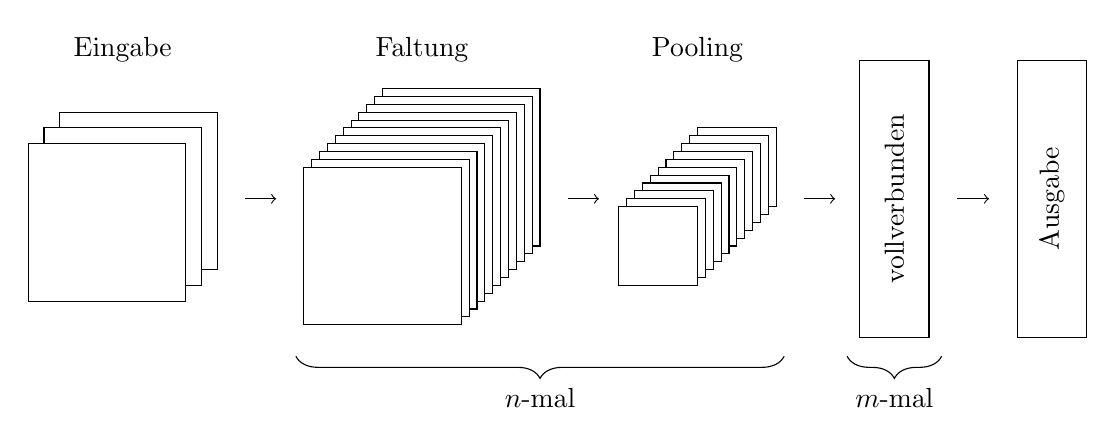
\begin{tikzpicture}
  \tikzstyle{node}=[rectangle, draw, minimum width=100pt, minimum height=25pt, inner sep=0pt, fill=white, rotate=90]
  \tikzstyle{rect}=[rectangle, draw, fill=white]
  \tikzstyle{path}=[->, shorten >= 10pt, shorten <= 10pt]

  % Eingabe.
  \draw[rect] (-0.1, 0.4) rectangle (1.9, 2.4);
  \draw[rect] (-0.3, 0.2) rectangle (1.7, 2.2);
  \draw[rect] (-0.5, 0)   rectangle (1.5, 2);

  % Faltung.
  \draw[rect] (4,   0.7)  rectangle (6,   2.7);
  \draw[rect] (3.9, 0.6)  rectangle (5.9, 2.6);
  \draw[rect] (3.8, 0.5)  rectangle (5.8, 2.5);
  \draw[rect] (3.7, 0.4)  rectangle (5.7, 2.4);
  \draw[rect] (3.6, 0.3)  rectangle (5.6, 2.3);
  \draw[rect] (3.5, 0.2)  rectangle (5.5, 2.2);
  \draw[rect] (3.4, 0.1)  rectangle (5.4, 2.1);
  \draw[rect] (3.3, 0)    rectangle (5.3, 2);
  \draw[rect] (3.2, -0.1) rectangle (5.2, 1.9);
  \draw[rect] (3.1, -0.2) rectangle (5.1, 1.8);
  \draw[rect] (3,   -0.3) rectangle (5, 1.7);

  % Pooling.
  \draw[rect] (8,   1.2) rectangle (9,   2.2);
  \draw[rect] (7.9, 1.1) rectangle (8.9, 2.1);
  \draw[rect] (7.8, 1)   rectangle (8.8, 2);
  \draw[rect] (7.7, 0.9) rectangle (8.7, 1.9);
  \draw[rect] (7.6, 0.8) rectangle (8.6, 1.8);
  \draw[rect] (7.5, 0.7) rectangle (8.5, 1.7);
  \draw[rect] (7.4, 0.6) rectangle (8.4, 1.6);
  \draw[rect] (7.3, 0.5) rectangle (8.3, 1.5);
  \draw[rect] (7.2, 0.4) rectangle (8.2, 1.4);
  \draw[rect] (7.1, 0.3) rectangle (8.1, 1.3);
  \draw[rect] (7,   0.2) rectangle (8,   1.2);

  \node at (0.7, 3.2) {Eingabe};
  \node at (4.5, 3.2) {Faltung};
  \node at (8,   3.2) {Pooling};

  \node[node] (1)  at (10.5, 1.3) {vollverbunden};
  \node[node] (2)  at (12.5, 1.3) {Ausgabe};

  \path[path] (1.9, 1.3) edge (3,    1.3);
  \path[path] (6, 1.3)   edge (7.1,  1.3);
  \path[path] (9, 1.3)   edge (10.1, 1.3);

  \path[path] (1) edge (2);

  \draw [decoration={brace,mirror,amplitude=8pt},decorate,-] (2.9,-0.7) -- node[below=8pt] {$n$-mal} (9.1,-0.7);
  \draw [decoration={brace,mirror,amplitude=8pt},decorate,-] (9.9,-0.7) -- node[below=8pt] {$m$-mal} (11.1,-0.7);
\end{tikzpicture}
  \caption[Netzarchitektur eines \glspl{CNN}]{Typische Netzarchitektur eines \glspl{CNN} bestehend aus beliebig vielen Faltungs- gefolgt von Poolingschichten.
  Die Abflachung der Merkmalskarten zu einem Vektor erlaubt die Verwendung beliebig vieler vollverbundener Schichten hin zur Ausgabe.}
\label{fig:cnn_aufbau}
\end{figure}


Eine Besonderheit des \glspl{CNN} ist weiterhin, dass sich die Receptive-Fields ihre Gewichte und Biaswerte teilen.
Damit erlernt ein Receptive-Field ein Merkmal, \zB{} eine Kante oder eine Textur, und findet dieses Merkmal auch in anderen Receptive-Fields, nur an unterschiedlichen Positionen~\cite{Nielsen}.
Das ermöglicht insbesondere das Erlernen translationsinvarianter Merkmale, die für eine Bilderkennung fundamental sind.
Aus diesem Grund spricht man auch häufig von einer \emph{Merkmalskarte} (\engl{} \emph{Feature-Map}), die durch eine Faltung über den Receptive-Fields entsteht.
Um mehrere Merkmale eines Receptive-Fields zu generieren, werden dabei üblicherweise eine Reihe von zusammengehörigen \emph{Eingabekarten} auf eine neue Menge von \emph{Ausgabekarten} projiziert.
Ein Bild $\gls{B} \in \gls{R}^{H \times W \times 3}$ mit drei Farbkanälen beschreibt \zB{} drei Merkmalskarten, die als Eingabe in das \gls{CNN} dienen.

Formal lässt sich damit die \emph{zweidimensionale Faltungsoperation}
\begin{equation*}
  \gls{conv2d} \gls{R}^{\colon H \times W \times M_{\mathrm{in}}} \to \gls{R}^{H \times W \times M_{\mathrm{out}}},
\end{equation*}
im Folgenden auch oft als \emph{klassische Faltungsoperation} betitelt, als
\begin{equation*}
  {\gls{conv2d}\left(\gls{B}\right)}_{yxm} \coloneqq \sum_{\Delta y = 1}^{F_y} \sum_{\Delta x = 1}^{F_x} \sum_{m_{\mathrm{in}} = 1}^{M_\mathrm{in}} \gls{B}_{y + \left\lceil F_y/2 \right\rceil - \Delta y, x + \left\lceil F_x/2 \right\rceil - \Delta x, m_{\mathrm{in}}} \gls{W}_{\Delta y, \Delta x, m_{\mathrm{in}}, m}
\end{equation*}
mit $1 \leq y \leq H$, $1 \leq x \leq W$ und $1 \leq m \leq M_{\mathrm{out}}$ definieren, wobei $\gls{B} \in \gls{R}^{H \times W \times M_{\mathrm{in}}}$ die Eingabe und $\gls{W} \in \gls{R}^{F_y \times F_x \times M_{\mathrm{in}} \times M_{\mathrm{out}}}$ den Filter \bzw{} Gewichtstensor der Faltungsoperation mit Filtergröße $F_y \times F_x$ von $M_{\mathrm{in}} \in \gls{N}$ Eingabekarten auf $M_{\mathrm{out}} \in \gls{N}$ Ausgabekarten beschreibt~\cite{tensorflow}.
Auf die Aufsummierung eines Bias $\gls{b} \in \gls{R}^{M_{\mathrm{out}}}$ sowie die Anwendung der Aktivierungsfunktion \gls{act} auf \gls{conv2d} wurde hier zur Vereinfachung verzichtet.
Der Wert eines Indexzugriffs auf die Eingabekarte \gls{B}, der über die Grenzen von \gls{B} hinausgeht, wird üblicherweise auf Null gesetzt (\emph{Zero-Padding}), sodass dieser keinen Einfluss auf die Faltung nimmt und die Ausgabekarte damit die gleiche Höhe und Breite der Eingabekarte besitzt~\cite{tensorflow}.
Eine Reduktion der Auflösung innerhalb der Faltungsschicht kann erreicht werden, indem nicht über jedes Neuron, sondern nur über eine Untermenge dieser in fester Schrittweite $s_y \times s_x$ zueinander gefaltet wird.
Eine Alternative dazu ist die Verwendung einer \emph{Poo\-ling\-sch\-icht}, die üblicherweise direkt nach einer Faltungsschicht zum Einsatz kommt und versucht, die Ausgabe der Faltungsschicht zu reduzieren \bzw{} auf das Wesentliche zu vereinfachen.
Eine Poolingoperation besitzt analog zu \gls{conv2d} eine Fenstergröße sowie eine Schrittweite.
Die beliebteste Poolingoperation ist das \emph{Max-Pooling}, welche sich jeweils für das Maximum der Aktivierungen innerhalb jedes Fensters entscheidet~\cite{Nielsen}.
Eine Poolingoperation mit Fenstergröße $2 \times 2$ sowie Schrittweite $2 \times 2$ reduziert damit die Daten der Merkmalskarte um genau die Hälfte.

Ein \gls{CNN} besteht typischerweise aus mehreren Faltungs- und Poolingschichten, sodass die Menge der Merkmalskarten dabei stetig erhöht und die Auflösung stetig verringert wird~\cite{Nielsen}.
Damit entstehen im späteren Verlauf des Netzes Merkmalskarten, die immer größere Receptive-Fields des Eingabebildes basierend auf den ermittelten Merkmalen vorangegangener Schichten beschreiben.
Nach einer gewissen Anzahl an Faltungen werden die Merkmalskarten zu einem Vektor umsortiert, sodass vollverbundene Schichten hin zur Ausgabe genutzt werden können~\cite{Nielsen}.
Abbildung~\ref{fig:cnn_aufbau} illustriert den üblichen Aufbau eines \glspl{CNN}.
\begin{figure}[t]
\centering
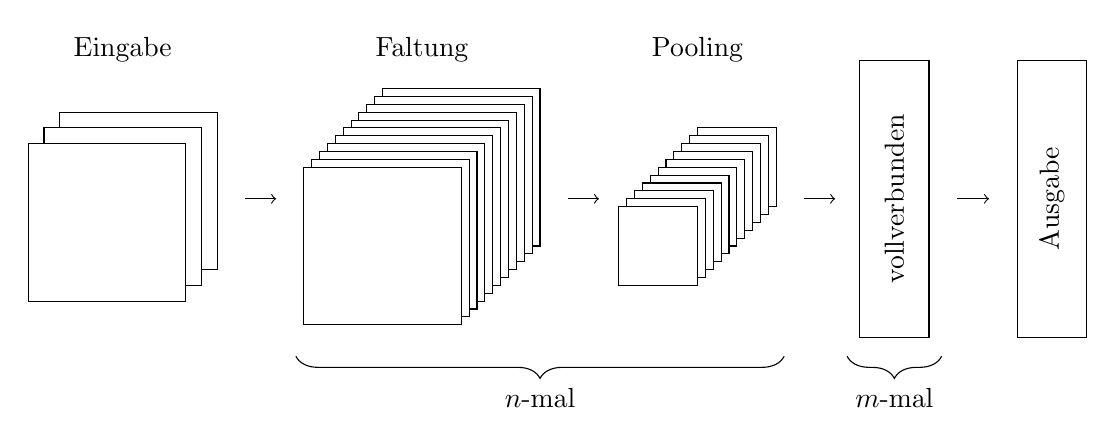
\begin{tikzpicture}
  \tikzstyle{node}=[rectangle, draw, minimum width=100pt, minimum height=25pt, inner sep=0pt, fill=white, rotate=90]
  \tikzstyle{rect}=[rectangle, draw, fill=white]
  \tikzstyle{path}=[->, shorten >= 10pt, shorten <= 10pt]

  % Eingabe.
  \draw[rect] (-0.1, 0.4) rectangle (1.9, 2.4);
  \draw[rect] (-0.3, 0.2) rectangle (1.7, 2.2);
  \draw[rect] (-0.5, 0)   rectangle (1.5, 2);

  % Faltung.
  \draw[rect] (4,   0.7)  rectangle (6,   2.7);
  \draw[rect] (3.9, 0.6)  rectangle (5.9, 2.6);
  \draw[rect] (3.8, 0.5)  rectangle (5.8, 2.5);
  \draw[rect] (3.7, 0.4)  rectangle (5.7, 2.4);
  \draw[rect] (3.6, 0.3)  rectangle (5.6, 2.3);
  \draw[rect] (3.5, 0.2)  rectangle (5.5, 2.2);
  \draw[rect] (3.4, 0.1)  rectangle (5.4, 2.1);
  \draw[rect] (3.3, 0)    rectangle (5.3, 2);
  \draw[rect] (3.2, -0.1) rectangle (5.2, 1.9);
  \draw[rect] (3.1, -0.2) rectangle (5.1, 1.8);
  \draw[rect] (3,   -0.3) rectangle (5, 1.7);

  % Pooling.
  \draw[rect] (8,   1.2) rectangle (9,   2.2);
  \draw[rect] (7.9, 1.1) rectangle (8.9, 2.1);
  \draw[rect] (7.8, 1)   rectangle (8.8, 2);
  \draw[rect] (7.7, 0.9) rectangle (8.7, 1.9);
  \draw[rect] (7.6, 0.8) rectangle (8.6, 1.8);
  \draw[rect] (7.5, 0.7) rectangle (8.5, 1.7);
  \draw[rect] (7.4, 0.6) rectangle (8.4, 1.6);
  \draw[rect] (7.3, 0.5) rectangle (8.3, 1.5);
  \draw[rect] (7.2, 0.4) rectangle (8.2, 1.4);
  \draw[rect] (7.1, 0.3) rectangle (8.1, 1.3);
  \draw[rect] (7,   0.2) rectangle (8,   1.2);

  \node at (0.7, 3.2) {Eingabe};
  \node at (4.5, 3.2) {Faltung};
  \node at (8,   3.2) {Pooling};

  \node[node] (1)  at (10.5, 1.3) {vollverbunden};
  \node[node] (2)  at (12.5, 1.3) {Ausgabe};

  \path[path] (1.9, 1.3) edge (3,    1.3);
  \path[path] (6, 1.3)   edge (7.1,  1.3);
  \path[path] (9, 1.3)   edge (10.1, 1.3);

  \path[path] (1) edge (2);

  \draw [decoration={brace,mirror,amplitude=8pt},decorate,-] (2.9,-0.7) -- node[below=8pt] {$n$-mal} (9.1,-0.7);
  \draw [decoration={brace,mirror,amplitude=8pt},decorate,-] (9.9,-0.7) -- node[below=8pt] {$m$-mal} (11.1,-0.7);
\end{tikzpicture}
  \caption[Netzarchitektur eines \glspl{CNN}]{Typische Netzarchitektur eines \glspl{CNN} bestehend aus beliebig vielen Faltungs- gefolgt von Poolingschichten.
  Die Abflachung der Merkmalskarten zu einem Vektor erlaubt die Verwendung beliebig vieler vollverbundener Schichten hin zur Ausgabe.}
\label{fig:cnn_aufbau}
\end{figure}


Eine Besonderheit des \glspl{CNN} ist weiterhin, dass sich die Receptive-Fields ihre Gewichte und Biaswerte teilen.
Damit erlernt ein Receptive-Field ein Merkmal, \zB{} eine Kante oder eine Textur, und findet dieses Merkmal auch in anderen Receptive-Fields, nur an unterschiedlichen Positionen~\cite{Nielsen}.
Das ermöglicht insbesondere das Erlernen translationsinvarianter Merkmale, die für eine Bilderkennung fundamental sind.
Aus diesem Grund spricht man auch häufig von einer \emph{Merkmalskarte} (\engl{} \emph{Feature-Map}), die durch eine Faltung über den Receptive-Fields entsteht.
Um mehrere Merkmale eines Receptive-Fields zu generieren, werden dabei üblicherweise eine Reihe von zusammengehörigen \emph{Eingabekarten} auf eine neue Menge von \emph{Ausgabekarten} projiziert.
Ein Bild $\gls{B} \in \gls{R}^{H \times W \times 3}$ mit drei Farbkanälen beschreibt \zB{} drei Merkmalskarten, die als Eingabe in das \gls{CNN} dienen.

Formal lässt sich damit die \emph{zweidimensionale Faltungsoperation}
\begin{equation*}
  \gls{conv2d} \gls{R}^{\colon H \times W \times M_{\mathrm{in}}} \to \gls{R}^{H \times W \times M_{\mathrm{out}}},
\end{equation*}
im Folgenden auch oft als \emph{klassische Faltungsoperation} betitelt, als
\begin{equation*}
  {\gls{conv2d}\left(\gls{B}\right)}_{yxm} \coloneqq \sum_{\Delta y = 1}^{F_y} \sum_{\Delta x = 1}^{F_x} \sum_{m_{\mathrm{in}} = 1}^{M_\mathrm{in}} \gls{B}_{y + \left\lceil F_y/2 \right\rceil - \Delta y, x + \left\lceil F_x/2 \right\rceil - \Delta x, m_{\mathrm{in}}} \gls{W}_{\Delta y, \Delta x, m_{\mathrm{in}}, m}
\end{equation*}
mit $1 \leq y \leq H$, $1 \leq x \leq W$ und $1 \leq m \leq M_{\mathrm{out}}$ definieren, wobei $\gls{B} \in \gls{R}^{H \times W \times M_{\mathrm{in}}}$ die Eingabe und $\gls{W} \in \gls{R}^{F_y \times F_x \times M_{\mathrm{in}} \times M_{\mathrm{out}}}$ den Filter \bzw{} Gewichtstensor der Faltungsoperation mit Filtergröße $F_y \times F_x$ von $M_{\mathrm{in}} \in \gls{N}$ Eingabekarten auf $M_{\mathrm{out}} \in \gls{N}$ Ausgabekarten beschreibt~\cite{tensorflow}.
Auf die Aufsummierung eines Bias $\gls{b} \in \gls{R}^{M_{\mathrm{out}}}$ sowie die Anwendung der Aktivierungsfunktion \gls{act} auf \gls{conv2d} wurde hier zur Vereinfachung verzichtet.
Der Wert eines Indexzugriffs auf die Eingabekarte \gls{B}, der über die Grenzen von \gls{B} hinausgeht, wird üblicherweise auf Null gesetzt (\emph{Zero-Padding}), sodass dieser keinen Einfluss auf die Faltung nimmt und die Ausgabekarte damit die gleiche Höhe und Breite der Eingabekarte besitzt~\cite{tensorflow}.
Eine Reduktion der Auflösung innerhalb der Faltungsschicht kann erreicht werden, indem nicht über jedes Neuron, sondern nur über eine Untermenge dieser in fester Schrittweite $s_y \times s_x$ zueinander gefaltet wird.
Eine Alternative dazu ist die Verwendung einer \emph{Poo\-ling\-sch\-icht}, die üblicherweise direkt nach einer Faltungsschicht zum Einsatz kommt und versucht, die Ausgabe der Faltungsschicht zu reduzieren \bzw{} auf das Wesentliche zu vereinfachen.
Eine Poolingoperation besitzt analog zu \gls{conv2d} eine Fenstergröße sowie eine Schrittweite.
Die beliebteste Poolingoperation ist das \emph{Max-Pooling}, welche sich jeweils für das Maximum der Aktivierungen innerhalb jedes Fensters entscheidet~\cite{Nielsen}.
Eine Poolingoperation mit Fenstergröße $2 \times 2$ sowie Schrittweite $2 \times 2$ reduziert damit die Daten der Merkmalskarte um genau die Hälfte.

Ein \gls{CNN} besteht typischerweise aus mehreren Faltungs- und Poolingschichten, sodass die Menge der Merkmalskarten dabei stetig erhöht und die Auflösung stetig verringert wird~\cite{Nielsen}.
Damit entstehen im späteren Verlauf des Netzes Merkmalskarten, die immer größere Receptive-Fields des Eingabebildes basierend auf den ermittelten Merkmalen vorangegangener Schichten beschreiben.
Nach einer gewissen Anzahl an Faltungen werden die Merkmalskarten zu einem Vektor umsortiert, sodass vollverbundene Schichten hin zur Ausgabe genutzt werden können~\cite{Nielsen}.
Abbildung~\ref{fig:cnn_aufbau} illustriert den üblichen Aufbau eines \glspl{CNN}.
\begin{figure}[t]
\centering
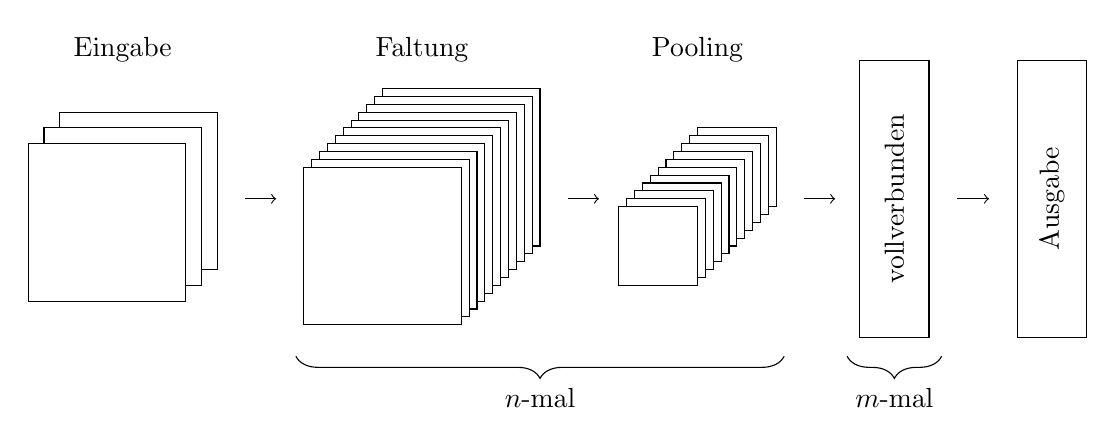
\begin{tikzpicture}
  \tikzstyle{node}=[rectangle, draw, minimum width=100pt, minimum height=25pt, inner sep=0pt, fill=white, rotate=90]
  \tikzstyle{rect}=[rectangle, draw, fill=white]
  \tikzstyle{path}=[->, shorten >= 10pt, shorten <= 10pt]

  % Eingabe.
  \draw[rect] (-0.1, 0.4) rectangle (1.9, 2.4);
  \draw[rect] (-0.3, 0.2) rectangle (1.7, 2.2);
  \draw[rect] (-0.5, 0)   rectangle (1.5, 2);

  % Faltung.
  \draw[rect] (4,   0.7)  rectangle (6,   2.7);
  \draw[rect] (3.9, 0.6)  rectangle (5.9, 2.6);
  \draw[rect] (3.8, 0.5)  rectangle (5.8, 2.5);
  \draw[rect] (3.7, 0.4)  rectangle (5.7, 2.4);
  \draw[rect] (3.6, 0.3)  rectangle (5.6, 2.3);
  \draw[rect] (3.5, 0.2)  rectangle (5.5, 2.2);
  \draw[rect] (3.4, 0.1)  rectangle (5.4, 2.1);
  \draw[rect] (3.3, 0)    rectangle (5.3, 2);
  \draw[rect] (3.2, -0.1) rectangle (5.2, 1.9);
  \draw[rect] (3.1, -0.2) rectangle (5.1, 1.8);
  \draw[rect] (3,   -0.3) rectangle (5, 1.7);

  % Pooling.
  \draw[rect] (8,   1.2) rectangle (9,   2.2);
  \draw[rect] (7.9, 1.1) rectangle (8.9, 2.1);
  \draw[rect] (7.8, 1)   rectangle (8.8, 2);
  \draw[rect] (7.7, 0.9) rectangle (8.7, 1.9);
  \draw[rect] (7.6, 0.8) rectangle (8.6, 1.8);
  \draw[rect] (7.5, 0.7) rectangle (8.5, 1.7);
  \draw[rect] (7.4, 0.6) rectangle (8.4, 1.6);
  \draw[rect] (7.3, 0.5) rectangle (8.3, 1.5);
  \draw[rect] (7.2, 0.4) rectangle (8.2, 1.4);
  \draw[rect] (7.1, 0.3) rectangle (8.1, 1.3);
  \draw[rect] (7,   0.2) rectangle (8,   1.2);

  \node at (0.7, 3.2) {Eingabe};
  \node at (4.5, 3.2) {Faltung};
  \node at (8,   3.2) {Pooling};

  \node[node] (1)  at (10.5, 1.3) {vollverbunden};
  \node[node] (2)  at (12.5, 1.3) {Ausgabe};

  \path[path] (1.9, 1.3) edge (3,    1.3);
  \path[path] (6, 1.3)   edge (7.1,  1.3);
  \path[path] (9, 1.3)   edge (10.1, 1.3);

  \path[path] (1) edge (2);

  \draw [decoration={brace,mirror,amplitude=8pt},decorate,-] (2.9,-0.7) -- node[below=8pt] {$n$-mal} (9.1,-0.7);
  \draw [decoration={brace,mirror,amplitude=8pt},decorate,-] (9.9,-0.7) -- node[below=8pt] {$m$-mal} (11.1,-0.7);
\end{tikzpicture}
  \caption[Netzarchitektur eines \glspl{CNN}]{Typische Netzarchitektur eines \glspl{CNN} bestehend aus beliebig vielen Faltungs- gefolgt von Poolingschichten.
  Die Abflachung der Merkmalskarten zu einem Vektor erlaubt die Verwendung beliebig vieler vollverbundener Schichten hin zur Ausgabe.}
\label{fig:cnn_aufbau}
\end{figure}

